\section{Niegripp bei Magdeburg}

\begin{figure}[h]
	\fbox{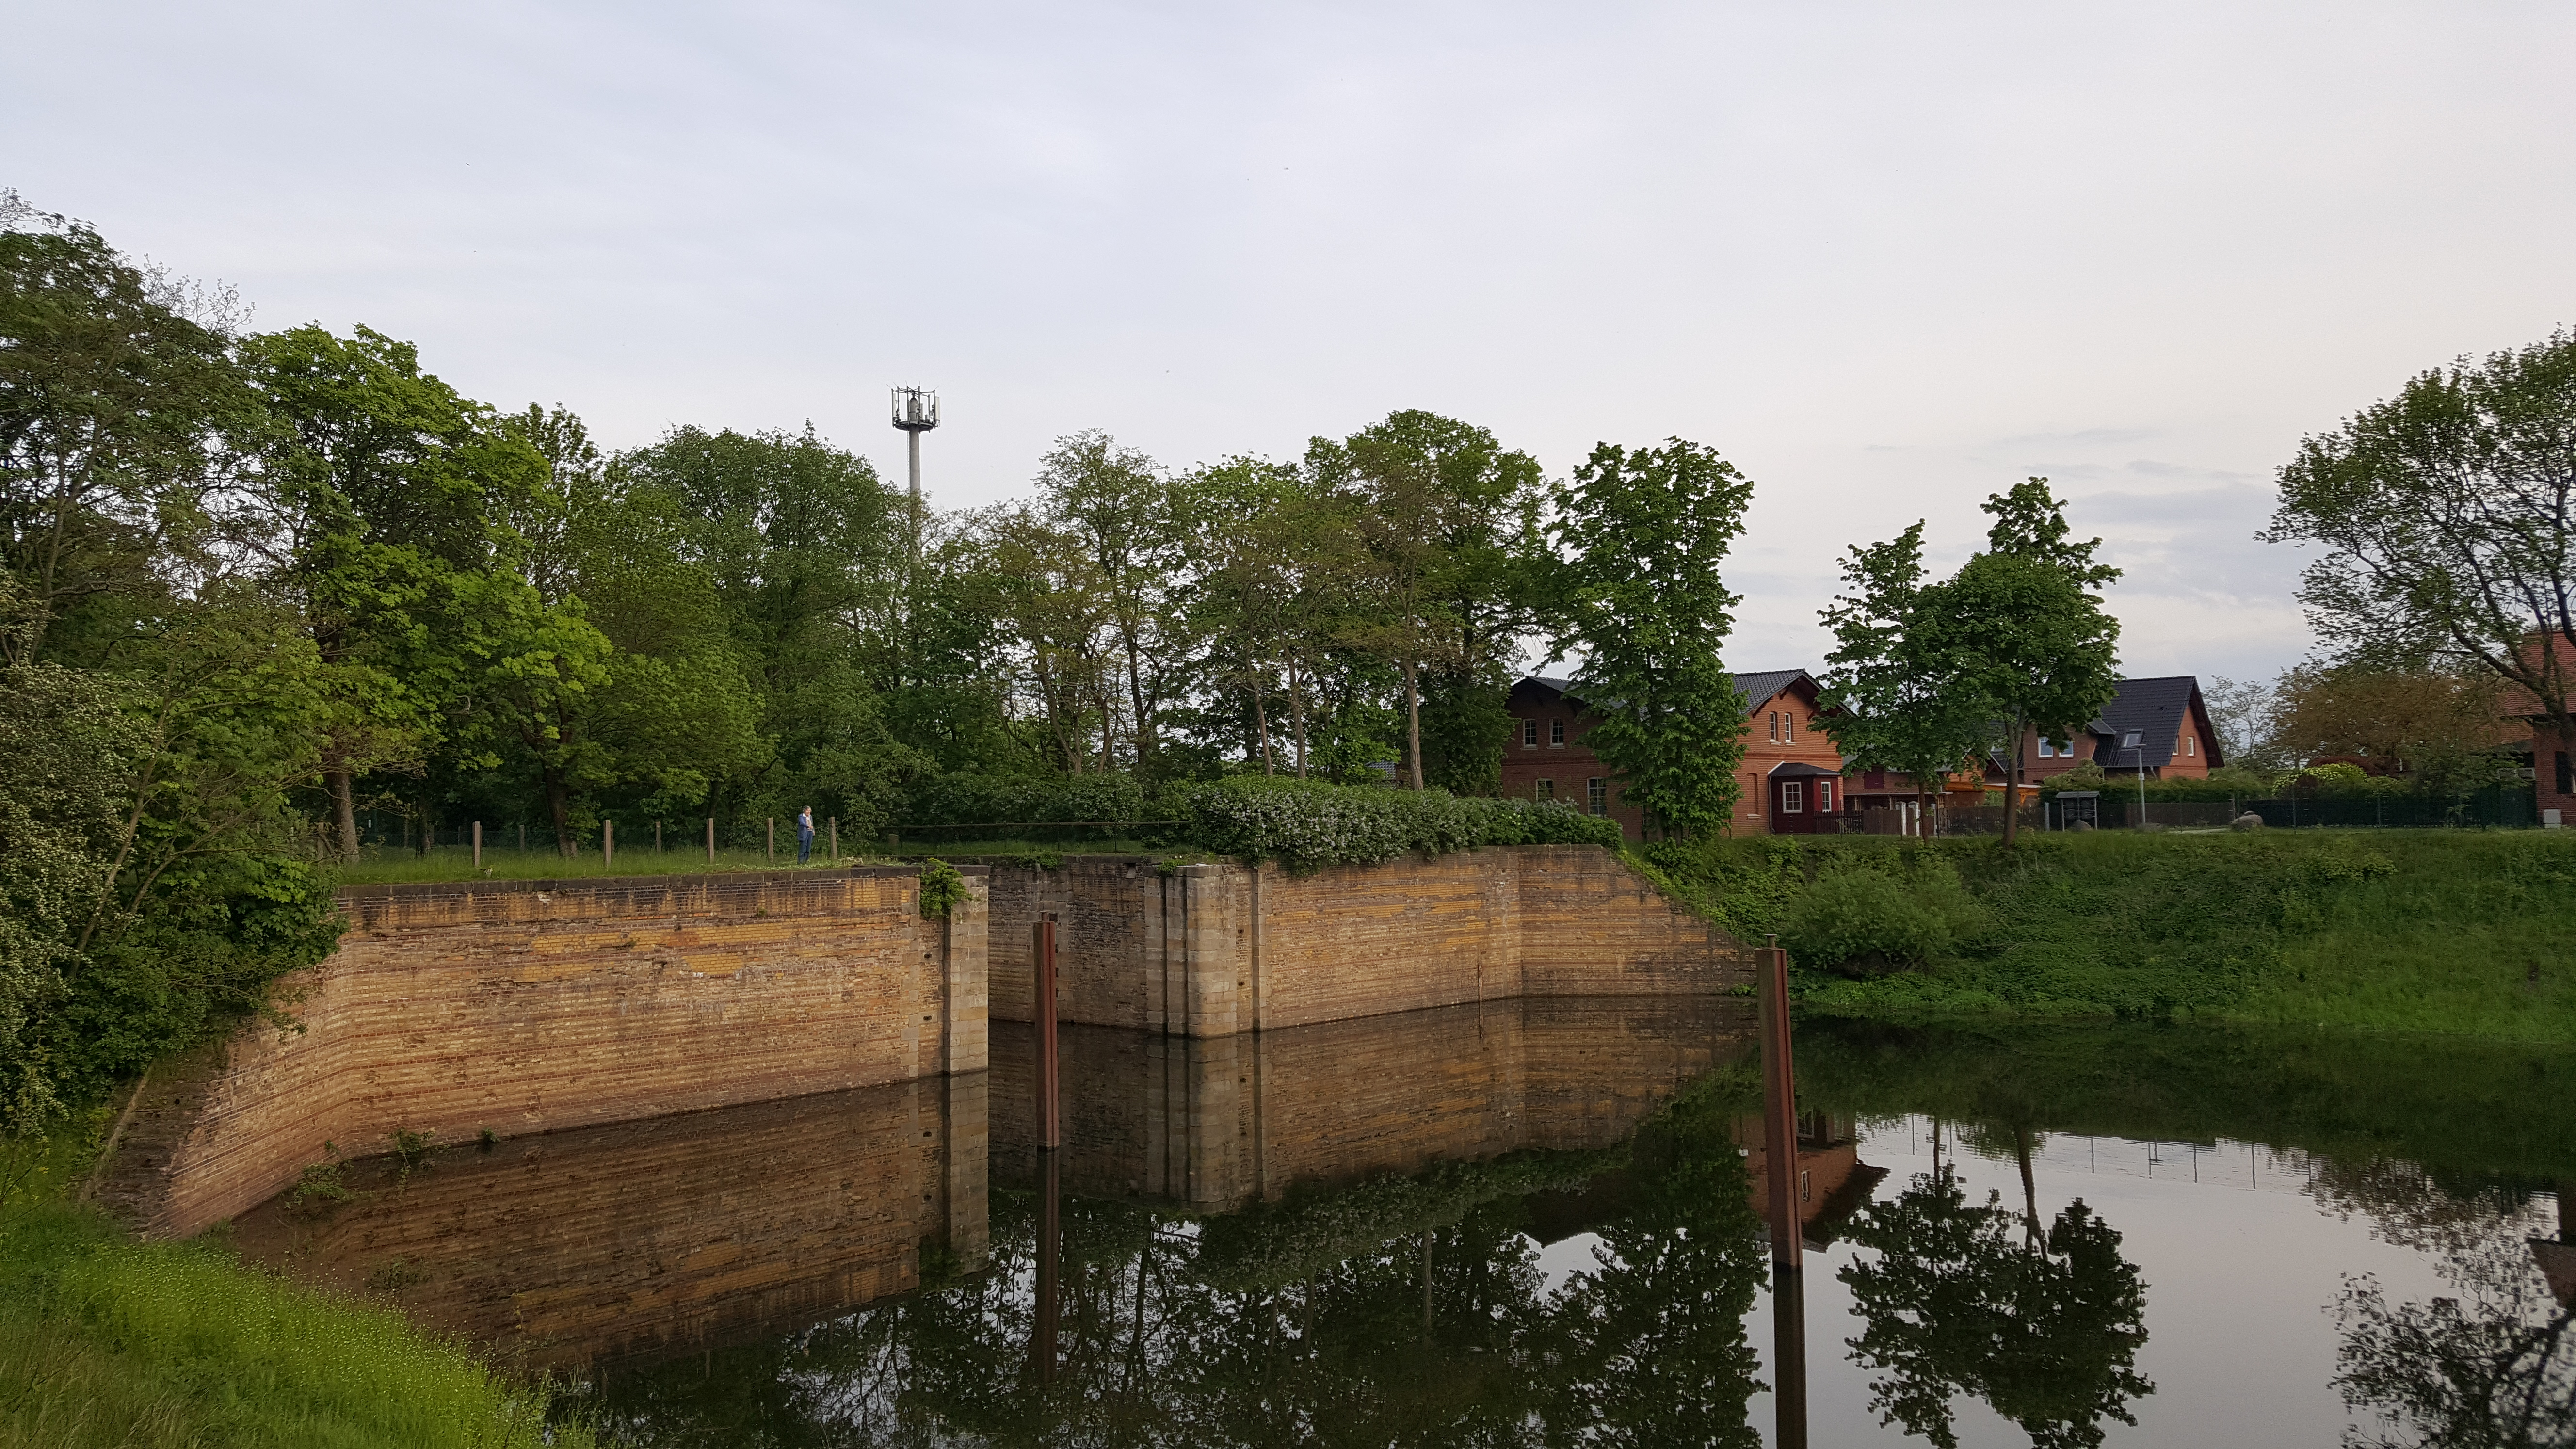
\includegraphics[width=\linewidth]{Photos/20210520_194728.jpg}}
	\caption{Alte Schleuse in Niegripp, Mai 2021}
	\label{fig:schleuse_niegripp}
\end{figure}

Der Schauplatz meiner Kindheit war Niegripp, da, wo der Ihlekanal in die Elbe mündet. Haus und Garten standen im Windschutz des hohen Elbedammes, der hier auslief in das Schleusenplateau, eine künstliche Aufschüttung mit den Häusern des Zolleinnehmers Wagner und des Schleusenmeister Zültz. Aus unserem Garten führte eine Treppe hinauf, und nach wenigen Schritten gelangte man zu einer stets nach frischem Brot und Bier riechenden Baracke, wo die Schiffer während oder vor dem Durchschleusen einkauften und sich erfrischten. Rechts davon ein großer Schuppen mit geteerten Balken, in dem es sich für Kinder bei Regenwetter herrlich saß. Am Schleusengehäuse und hinter unserem Garten führten zwei steile Steintreppen hinab zum Kanal. Dieses ganze Gelände war ein herrlicher Tummelplatz und wurde in meiner frühen Kindheit argwöhnisch vom Schleusenmeister Zültz und vom einarmigen Kanalaufseher Timmermann, einem Veteran des Krieges 1870/71, bewacht; in ihnen sah ich meine natürlichen Feinde, denn beide stellten ein fürchterliches Gebrüll an, wenn ich die Treppen zum Kanal hinab oder über den allerdings für Kinder nicht geschützten Schleusensteg gehen wollte.

Meine Mutter hatte hier viele unsichtbare Verbotstafeln errichtet, und ich beneidete manchmal meine Freunde Gustav und Otto Lüdde, die solche Verbote nicht zu kennen schienen. Denn die Erziehung des \enquote{Ungi} und der dreieinviertel Jahre jüngeren Ella lag wesentlich in den Händen meiner Mutter. Mein Vater, damals \enquote{Königlicher Hilfsförster} im Dienste der Hausfideikommisverwaltung der Hohenzollern, war ein tüchtiger Forstmann, leidenschaftlicher Jäger und Heger sowie erfolgreicher Imker. Er war wenig zu Haus, ich erlebte ihn aber täglich bei den Mahlzeiten, ausgenommen das Frühstück.

Wenn er nicht im Dienst oder auf Jagd war -- was beides praktisch ineinander überging oder zusammenfiel, sah ich ihn an seinem Fahrrade basteln oder in der Bienenhütte werken. Er hatte eine Art selbständiger Wasserleitung in den Bienenkörben konstruiert und, wie ich noch 1949 in Niegripp hörte, auf einer Imkerausstellung in Genthin vorgeführt; er hat auch in Burg bei Magdeburg gelegentlich Vorträge über Fragen der Imkerei gehalten.

Ich erinnere mich, wie er einmal von meiner Mutter, immer wieder aufs Blatt schauend, den Vortrag auf Probe sprach, während sie ihn gelegentlich mit stilistischen Verbeserungsvorschlägen unterbrach. Da mein Vater meine Freiheit weniger einschränkte, erschien mir in der Frühzeit meine Mutter als der strengere Elternteil. Da sich in ein - zwei Fällen, wohl im Alter zwischen 5 und 7 Jahren, gezeigt hatte, dass ich nicht, wie sie es wollte, jede Mahlzeit der Erwachsenen vertrug, erklärte sie, ich hätte einen \enquote{schwachen Magen} und bekam (daher), ich glaube mit Ella, Diätkost: außer Wild wenig Fleisch, keine Wurst, kein Weiß- und übliches Roggenbrot, nur Schrotbrot mit Apfelscheiben und ein Glas Milch zum Abendbrot. Wenn meine Mutter krank oder zu ihren Verwandten nach Österreich oder Ungarn verreist war, was in der Niegripp-Zeit wohl jedes Jahr vorkam, wurde ich von unserem langjährigen, tüchtigen, auch eigenwilligen Dienstmädchen durch interessantere Kost mit Roggenbrot und sogar warmem Abendbrot, das mir ausgezeichnet bekam, entschädigt. Mittags, vor dem Essen, schlich ich gern in der Küche herum, denn meine Mutter gab ihrem \enquote{Ungi} (wie ich mich selbst nannte) eine Keule von dem \enquote{Fan} d.h. Fleisch, und zwar von dem in der Pfanne gebratenen Wildgeflügel; besonders Wildentenkeulen schätzte ich sehr.

Übrigens behielt ich meine private Kindersprache, wie ich glaube, lange bei, wohl bis zum vollendeten 5. Lebensjahr, da meine Eltern im Gespräch mit mir sich ebenfalls vieler meiner Privatvokabeln bedienten. Das entsprach übrigens ganz dem Standpunkt der damaligen Alterstufen-Psychologie; noch William Stern, Philosophieprofessor in Breslau, später Hamburg, lehrte 1913, die Kindersprache sei ein ehrwürdiges Produkt kindlicher Sprachschöpfung, das frühzeitig zu unterdrücken kein Anlass bestehe. Ich kann mich nur noch an wenige Wörter erinnern wie Fau (Fleisch), Gridika (Zigarre), Zang (Zeitung).

Meine Schwester, die als Mädchen sehr früh eine \enquote{eigene} Sprache entwickelte, nannte sich selbst \enquote{Miedi} und mich den \enquote{Biedi}. Wenn wir zusammen spielten, redeten wir uns so an bis ich mit 6 Jahren in die Schule ging, und ich übernahm manche Ausdrucksformen Ellas, die ich jedoch vergessen habe. Mit 5 Jahren spätestens hatte ich die Kindersprache abgelegt und sprach Hochdeutsch, während meine Gespielen vorwiegend platt (niederdeutsch) redeten. Im 4. Lebensjahr brachte mir die bei uns mit dem Opa wohnende \enquote{Oka} (Großmutter mütterlicherseits) die Uhrzeit bei. Auf einem Schränkchen (Vertiko) im Wohnzimmer stehend betrachtete ich das Zifferblatt des Regulators und stellte fest: \enquote{Es ist bald 4 oder es ist 6 durch}; die Minuten konnte ich erst zwischen 5 und sechs Jahren bestimmen. In Anwesenheit von Gästen hob man mich auf das Vertiko und mein Können wurde bewundert, \enquote{was mir genehm war}.

Bei uns wohnten Mutters Eltern; er \enquote{der Opa} hatte ein verschuldetes Gut ererbt, es frühzeitig verkauft und war Gutsinspektor bei irgendeinem Magnaten gewesen. Seinen beiden Kindern konnte er für damalige Verhältnisse eine ausgezeichnete Ausbildung geben, meiner Mutter die Erziehung in der Herrnhuter Töchterschule Kleinwelka bei Bautzen (einem Internat) -- die entsprechende Jungenschule hatte einst Fürst Pückler-Muskau besucht. Ihr Bruder besuchte das Görlitzer Wilhelm-Gymnasium, studierte Jura und wurde angesehener Rechtsanwalt und \enquote{Justizrat} in Görlitz. Dessen Sohn Walter -- mein mir etwa gleichaltriger Vetter -- wurde ebenfalls Jurist und stieg 1934 als tüchtiger Finanzsachverständiger zum Generaldirektor der Hapag auf, deren Aktienmehrheit nach dem 1. Weltkrieg meines Wissens in amerikanischen Händen lag.

Opa ging viel mit mir spazieren und vermittelte mir u.a. landwirtschaftliche Kenntnisse. So lernte ich im Vorschulalter die jungen Saaten nach Roggen, Weizen, Hafer, Gerste unterscheiden, was ich später und heute nicht mehr konnte. Man amüsierte sich, wenn ich vor Erwachsenen, so auch vor dem späteren Lehrer und Kantor, naseweise Äußerungen über Fleiß bzw. Faulheit der Bauern, Ordnung und Unordnung etc. der Felder tat. Er erklärte, ich sei \enquote{wissbegierig} während er bei meiner Schwester -- zu Unrecht -- nur \enquote{Neugier} diagnostizierte. Ich war der Verzug meiner Großmutter, der \enquote{Oka}, deren letzte Worte übrigens \enquote{der Ungi} gewesen sein sollten. Beide Großeltern starben kurz hintereinander mit 70 Jahren an Lungenentzündung. Ich erinnere mich, dass eines Abends der Arzt aus Burg in seiner Droschke kam, nach den Untersuchungen bedauernd \enquote{beginnende Lungenentzündung} sagte, und darauf meine Mutter still weinte. Das war 1900 bzw. 1901 das medizinische Todesurteil, denn damals gab es noch kein wirksames Medikament gegen Lungenentzündung, eine Krankheit, die um 1900 noch zu den häufigsten Todesursachen zählte.

\label{para:kindheitserinnerungen}Zu meinen frühesten Kindheitserinnerungen zählen folgende: In meiner Kindheit fanden in und bei Niegripp mehrfach Manöver Magdeburger Truppenteile statt: Pioniere bauten eine Pontonbrücke über die Elbe, Ulanen\footnote{Ulanen sind eine mit Lanzen bewaffnete Gattung der Kavallerie} ritten auf dem ausgedehnten Elbanger Attacken z.B. gegen feuernde Artillerie. Die Eltern gingen mit ihren kleinen Kindern zur Elbe und über die Pontonbrücke nach Heinrichsberg, der Schulunterricht fiel aus, die Klassen gingen mit Kantor und Lehrer ebenfalls zur Elbe. Ich hatte das 3. Lebensjahr vollendet, als ein solches Manöver mit Ulanen und Artillerie stattfand. Es ertönten gewaltige Kanonenschläge, man sprach viel von den Ulanen. Am nächsten Tage gab es bei uns zum Mittagessen Rouladen -- ich verstand Ulanen, glaubte, wir essen die totgeschossenen Ulanen auf; es bedrückte mich, ich wagte aber nicht, die erlösende Frage an die Eltern zu richten. Ein Jahr später wusste ich wohl schon, dass die Kanonen zwar sehr laut donnern, aber nichts Böses anrichten. Ich hatte aber, wie alle Dorfkinder, große Angst vor Gewittern. Einmal, an einem heißen Sommertag, donnerte es unaufhörlich aus einer dunklen Wolkenwand jenseits des Kanals. Meine Mutter und das Dienstmädchen putzen im Garten Gemüse und pellten Erbsen aus. Ich hatte fürchterliche Angst und wollte ins Haus flüchten, sollte aber draußen bleiben. Ich war erst beruhigt, als der Schleusenmeister (natürlich auf Bitten meiner Mutter) mit lauter Stimme verkündete: \enquote{Das ist nur Kanonendonner!}

Meine Mutter erzog mich zum Gehorsam, bekämpfte jedoch mit unnachsichtiger Strenge die Lüge. Im Herbst lasen wir, die beiden Lüddes und ich, unter dem Nussbaum Walnüsse auf. Wir schlugen auch mehrere auf und aßen sie, ich auch, trotz strengen Verbots (wegen meines angeblich schwachen Magens). Meine Mutter musterte darauf misstrauisch meine Mundpartie und fragte: Fritz, hast du Nüsse gegessen? Aus Angst vor Strafe log ich: Nein! Sie rief meine Kumpanen herbei und fragte: \enquote{Habt ihr Nüsse gegessen?} \enquote{Ja}. \enquote{Hat Fritz Nüsse gegessen?} \enquote{Ja} Nun holte sie die Hundepeitsche, legte mich übers Knie und verdrosch mich, allerdings ohne besonders stark aufzudrücken. Den ganzen Tag über ließ sie mich spüren, dass ich mit der Lüge etwas sehr Verwerfliches getan hatte.

Lebhaft interessierte mich früh der Fischfang, vor allem das Angeln. Ich beneidete Erwachsene und größere Jungs, die ich im Kanal nahe der Schleuse hinter unserem Garten angeln sah. Mit meinem Freunde Gustav Lüdde zusammen hatte ich eine Angelrute gebastelt. Eines Tages eilte ich mit ihr über das Schleusentor und jenseits die Treppe herunter ans Kanalwasser. Als Köder hatte ich ein Brotklümpchen verwandt. Es biss kein Fisch an. Plötzlich brüllte mich von hinter über mir der einarmige Kanalaufseher mit schrecklicher Stimme an. Ich zog mit Schwung die Leine aus dem Wasser, der Angelhaken verfing sich im Regenschirm Timmermanns, dessen Gepolter wurde noch schlimmer; schließlich riss ich den Haken los und rannte, während sich ein warmer Strom über Bein und Hose ergoss, angsterfüllt nach Hause. Die wahrheitsgetreue Schilderung des Vorgangs und wohl auch das Komische meiner Situation bewahrten mich vor Strafe.

Im Sommer vor meinem Eintritt in die Schule starb Bismarck; ich erinnere mich sehr genau daran: 14 Tage lang läuteten von 12-13 Uhr mittags die Glocken. Erstmalig in meinem Leben, so glaube ich, ergriff mich ein Gefühl der Trauer, vor allem auch genährt durch Gespräche der Eltern. Der große Mann, dem wir alle so viel zu verdanken hatten, der nur an das Wohl unseres Landes dachte, und den der undankbare Kaiser fortgeschickt hatte, war tot. Sein Bild hing, außer einem großen Farbstich von Versailles \enquote{Vue générale, prise du bassin d'Appolon} und Photographien von Verwandten, im Wohnzimmer. Es wurde später durch eine schöne Farbreproduktion eines Bildes von Lenbach ersetzt. Den Farbstich von Schloss und Park Versailles hatten meine Großeltern mütterlicherseits von einer patriotischen Erbauungsreise nach Paris und Versailles (Spiegelsaal!) mitgebracht. Meine Eltern hatten in den 90-er Jahren eine Verlobungsreise zum Hermannsdenkmal im Teutoburger Wald gemacht.

Nach dem Eintritt in die Volksschule wurde ich mit des Lebens ganzem Jammer konfrontiert: der Rohrstock war wichtigstes Erziehungsinstrument. Er verging wohl keine Stunde, in der nicht einer von uns Jungen mit dem Stock unter jämmerlichem Geschrei verprügelt wurde. Lehrer Witte legte die Jungs über eine der vorderen Bänke oder ein Bein auf die Bank stützend über das Knie, wobei dann das Opfer oft schrie \enquote{ich falle} -- er darauf boshaft lachend erwiderte \enquote{nein, Bürschchen, ich halte dich fest!} Meine Eltern erfuhren vom Lehrer, dass ich weich veranlagt sei, da ich jedes Mal aus Mitleid mitweinte!

In der ersten Rechenstunde hatte ich einen großen Erfolg: ich konnte als Einziger der ca. 30 Schulanfänger bis 100 zählen. \enquote{Fritz, kannst du noch weiter zählen?} Ich bejahte stolz. \enquote{Einhundert, zweihundert, dreihundert.} Lehrer Witte lehnte dies jedoch kommentarlos zu meiner Enttäuschung ab.

Der tägliche ausgedehnte Religionsunterricht wurde wegen der damit verbundenen Hausaufgaben: Auswendiglernen langer alttestamentarischer Geschichten mit befremdlichen Namen wie Abraham, Melchisedek, Obadja etc. etc. und vieler Liederstrophen als lästig empfunden. Meine Mutter griff helfend ein: sie ging mit mir am windgeschützten Ihlekanal spazieren, sprach Sätze und Strophen vor und paukte sie mir ein. Im Religionsunterricht lernte ich u.a., dass es der liebe Gott besonders schätzt, wenn man ihm zu Ehren Lobgesänge anstimmt. Meine Mutter hatte mich zwar frühzeitig beten gelehrt, pflegte mit mir aber keine religiösen Gesänge. So hielt ich es für nötig, allein Gott den Herrn singend zu preisen, schämte mich aber vor meinen Eltern. So sang ich abends, gelegentlich auch morgens leise unter der Bettdecke.

Als ich acht Jahre alt war, kühlte sich mein bisher inniges Verhältnis mit dem lieben Gott plötzlich vorübergehend ab; das kam so: über dem Spiel hatte ich eine der Hausaufgaben ganz vergessen, nämlich drei Strophen eines Kirchenliedes auswendig zu lernen. Ich erschrak, als mir dies kurz vor dem Einschlafen einfiel. Faulheit und Vergessen wurden gleichermaßen mit dem Rohrstock geahndet. Da kam mir ein rettender Gedanke: in letzter Zeit waren die Eigenschaften Gottes herausgearbeitet worden, voran Allmächtigkeit und Allgüte. Ich wusste, dass Gott ein inbrünstiges Gebet erfüllt. So flehte ich ihn recht innig an, er möge machen, dass ich am nächsten Morgen beim Erwachen die befohlenen drei Strophen schön auswendig hersagen kann; ich versäumte auch nicht, mein inbrünstiges Gebet mit einem leisen Lobgesang des Herrn unter der Bettdecke zu beschließen -- und schlief vertrauensselig ein. Wie groß war meine Bestürzung und Enttäuschung beim Erwachen, dass mich der liebe Gott schmählich im Stich gelassen hatte und ich konnte nicht eine einzige Zeile hersagen. Das nahm ich ihm sehr übel und stellte für mehr als eine Woche Gebete und Lobgesänge ein.

Das alte Vertrauensverhältnis stellte sich erst später nach folgendem Vorfall wieder völlig her: im Herbst hatte ich eine Leiter an die mit Weinreben bedeckte Südwand des Forsthauses geschleppt; ich wollte mit meinem Taschenmesser ein paar Reben schneiden; oben stehend entglitt mir das Messer, ich suchte und suchte lange, im Wein, auf der Erde -- es war weg, nicht zu finden. Für einen Jungen damals ein sehr schmerzlicher Verlust! Ich richtete, noch auf der Leiter stehend, einen Hilferuf an Gott, und wiederholte mein Flehen im Abendgebet. Und siehe da! Am nächsten Morgen lag mein Messer auf dem Fensterbrett im Wohnzimmer! Ich war vom persönlichen Eingreifen Gottes überzeugt.

Im Sommer des wohl gleichen Jahres rauchte ich meine erste Zigarre. Die Eltern waren wie jeden Sonntag zur Kirche gegangen, das Mädchen arbeitete in der Küche, die Luft war rein; ich holte aus der eben angefangenen Kiste meines Vaters eine dicke Zigarre, nahm Streichhölzer, lief durch den Garten zur Böschung des Schleusenplateaus, schnitt wie der Vater die eine Spitze ab und zündete sie an, tat einige Züge, der Rauch kratzte scheußlich im Halse, so dass ich die brennende Zigarre ins Gras warf. Vater entdeckte alsbald die Lücke in der Kiste, sein Verdacht fiel sofort auf mich, ich gestand alles. Mein Vater schien eher belustigt als entrüstet.

Das wichtigste Spielzeug eines etwa 5-8 Jahre alten Dorfjungen war damals: im Frühjahr selbstgefertigte \enquote{Flitzbogen} mit Holzpfeilen, deren Enden einen aufgesetzten Kolben aus Holunder erhielten. Man fertigte Pfeifen aus saftigen Weidenruten, die mit dem Messerrücken weich geklopft wurden, so dass man das eingekerbte Holz aus der Rinde lösen konnte. Mit etwa acht Jahren spielte man mit einem großen Holzreifen, den man mit einem kurzen Holzstück schnell fortbewegte. Im März-April spielte der Holzkreisel eine Rolle; man schlug auf Fußwegen oder ebenen Fahrwegen auf ihn ein, man hatte gern zwei oder drei verschieden gefärbte Kreisel. Luxus waren schon summende Brummkreisel, Geschenke von Verwandten aus Berlin. Auch Spiele mit \enquote{Schnappkugeln} aus Glas oder gefärbtem Ton waren beliebt.

Ein großes Ereignis waren jedes Jahr die Sedanferien\footnote{der Sedantag war bis 1918 ein Feiertag anlässlich der entscheidenden Schlacht im Deutsch-Französischen Krieg 1870/71}. Eingeleitet wurden sie am Vorabend nach Einbruch der Dunkelheit durch Zapfenstreich. Voran die Dorfkapelle, gefolgt von der Bevölkerung und vor allem der Kinder mit Lampions; am schönsten war der Marsch auf dem Elbdamm und der Rundmarsch auf dem Schleusenplateau. Der Zug hielt vor dem Gutshaus, dem Pächter der zum königlichen Hausfideikommiss gehörenden Domäne der -- soweit eine solche vorhanden war -- die wichtigste Persönlichkeit des Dorfes war, nicht etwa Pastor oder Kantor. Er hielt die patriotische Ansprache mit dem Hoch auf Seine Majestät. Am nächsten Tag war schulfrei: Nachmittags und abends fanden auf dem Anger unter \enquote{den großen Eichen} Spiele für die Schulkinder statt, auch Blindekuh, Sackhüpfen und allerlei Wettspiele gehörten dazu. Die Kapelle spielte Märsche und Heimatlieder. Männer und Jugendliche drängten sich um eine Schießbude. Abends wurde im Saale des Gasthofs \enquote{Zum grünen Baum} getanzt.

Vor allem im Sommer lungerten wir Jungs viel an der Kanalschleuse herum und beobachteten den Dampferverkehr auf dem Kanal; wie die heutige Jugend jede Automarke kennt, so kannten wir die Namen der Dampfer, bevor sie mit eingeholtem Schornstein die Kanalbrücke passierten \enquote{Da kommt die Emma!} \enquote{Döskop; dat is doch die Schnakenburg.}

Den Verkehr auf der Elbe beobachteten wir vom Damm aus. Die großen Elbkähne, die oft in langen Schleppzügen von bis zu 22 Schiffen fuhren, zogen bei günstigem Winde ihre großen weißen Segel auf. Wir knüpften Bekanntschaften mit Schifferkindern der oft nur für wenige Stunden in Niegripp vor Anker gehenden Kähne an.

Ein großartiges Schauspiel war das nicht seltene Hochwasser der Elbe. Wenn das Wasser vormittags stieg, die Chaussee zum Fährhaus überflutete und sich rauschend in die tief gelegenen \enquote{Kolke} ergoss -- der \enquote{Heller} war nur 150~m von unserem Haus entfernt, der \enquote{Schweinebolk} 500~m -- fiel der Unterricht aus. Der Lehrer begab sich mit uns Schülern auf den Damm und dicht an die hereinbrechenden Fluten.

Hochwasser im Winter: Papa ließ im \enquote{Bauernbusch} Holz schlagen für Faschinen\footnote{Faschinen sind walzenförmige Reisig- bzw. Rutenbündeln von einigen Metern Länge, welche in erster Linie zur Abwehr von Erosionserscheinungen genutzt werden}. Unter seiner Leitung wurden die schwachen Stellen in Eile befestigt. Ich erinnere mich an eine unruhige Nacht, in der mein Vater verkündigte: Hochwasser um weitere 20 cm gestiegen und schließlich erlösend: 5 cm gefallen, Dammbruch bei Hohenwarte 7~km oberhalb Niegripp.

Im Winter tummelte man sich auf dem Eise -- mit 7 Jahren bekam ich Schlittschuhe. Bei hohem Schnee wurde ich in den ersten Schuljahren dicht vermummt auf einem Schlitten mit Rücklehne in die Schule gefahren, damit ich nicht kalte oder gar nasse Füße bekäme.

Im Winter 1900/1901 nahmen uns die Eltern zu einem 14-tägigen Aufenthalt in Berlin mit. Ich erinnere mich deutlich an die Bahnfahrt durch die tief verschneite Landschaft, an das rätselhafte Auf und Ab der Telegraphendrähte vor dem Abteilfenster und in Berlin natürlich vor allem an die vielen Pferdebahnen auf den Straßen und an die noch nicht so zahlreichen elektrischen Straßenbahnen, über denen an den Drähten so oft die bläulich blitzenden Funken sprühten. Ich soll oft \enquote{quengelich} und \enquote{unleidlich} gewesen sein, so besonders wenn wir mit einem Pferdevehikel fuhren, statt mit der Elektrischen. Mit einem Pferdevehikel fuhren wir ja schließlich auch von Niegripp nach unserer Kreisstadt Burg. Überwältigend war der Eindruck vom damals größten Warenhaus Berlins, Wertheim in der Leipziger Straße.

Einmal stand mein Vater mit mir vor der Berliner Haupt-Feuerwache. Bald ertönte ein schrilles Klingelzeichen, ein großes Tor öffnete sich, und heraus kam im Karacho die große von sechs Pferden gezogene Feuerspritze. Von den Verwandten, mit denen wir zusammen kamen, erinnere ich mich vor allem an Tante Martha Dehnicke, von Beruf Lehrerin, eine Cousine meiner Mutter, die erste Frau, die ich oft rauchen sah, was mir damals imponierte. Sie war überdies wegen ihrer erlesenen Geschenke, meist mit einem \enquote{Pfiff}, bei uns Kindern besonders gut angeschrieben. Später heiratete sie ihren Vetter Dr. Hans Dehnicke, nachmals Universitätsprofessor für Chemie an der Berliner Universität.

Im Sommer des gleichen Jahres, 1901, in dem mein Großvater Kurt Hoffmann, der mich oft auf seinen Spaziergängen mitgenommen hatte, gestorben war, hatte ich das Erlebnis der \enquote{ersten Liebe}. Sie hieß Anna Schmidt, war wie ich 8 Jahre alt, aus Magdeburg-Sudenburg und drei Ferienwochen zu Besuch in einem Nachbarhause. Wir fanden sofort aneinander Gefallen. Wir spielten täglich miteinander, trieben uns auf dem Anger herum, planschten im \enquote{Heller}, angelten zusammen. War ich mit Anna zusammen, störte mich die Anwesenheit meiner Niegripper Spielgefährten, einschließlich meiner Schwester Ella. Ich erfand Vorwände, um die anderen Jungen von uns fernzuhalten. Wir wussten einander stets viel zu erzählen. Mich interessierte Annas Leben und Magdeburg. Schließlich kam der Abschied. Er fiel uns schwer. Anna fuhr mit dem kleinen Dampfer, mit dem sie gekommen, eines Vormittags wieder zurück nach Magdeburg. Ich stand lange an dem Buhnenkopf, an dem der Dampfer angelegt hatte, und winkte und winkte, bis das Schiffchen zu einem Punkt mit einer schwachen Rauchfahne darüber zusammengeschrumpft war. Meine traurige Stimmung hielt mehrere Tage an. Nach einigen Wochen kam aus Sudenburg eine mit ungeübter Kinderhand geschriebene Karte, deren Inhalt ich wieder und immer wieder las: \enquote{Denkst du auch noch an mich? Ich denke aber an Dich. Deine Anna Schmidt}. Ich habe sie nie wieder gesehen.

Im gleichen Sommer, etwas später, verbrachten zwei Verwandte Kurt und Wilhelm Bertling aus Aachen ihre Ferien beim kinderlosen Ehepaar Wagner, Schleusenzoll Einnehmer wohnhaft auf dem Schleusenplateau, zwei nette mit mir gleich bzw. zwei Jahre ältere Jungen. Lebhafte, gepflegte Großstadtjungen, denen ich manche Anregung verdankte. Beide trugen schöne baumwollene Spielanzüge und Sandalen. Meine Mutter ließ mich im Sommer barfuß laufen (\enquote{das ist gesünder}), auf meine Kleidung verwandte sie geringe Sorgfalt (ich hatte einen \enquote{Paradeanzug} für Sonn- und Festtage, den ich hasste, da ich praktisch in ihm nicht frei spielen konnte.)

In der Gegenwart der Bertling-Jungen fühlte ich mich wegen der modernen Bekleidung frustriert. Mein Vater erklärte mir zwar, die Bertling-Jungen kämen von weither, von der Reichsgrenze, aber hier, unweit Berlins, der Residenz des Kaisers, könne man nicht so gekleidet gehen -- doch das überzeugte mich nicht. Einmal, als ich barfuß in Hemd und Hose im Garten spielte und plötzlich die beiden Bertlings schick angezogen die Treppe vom Schleusenplateau heruntersteigen sah, kam es zu einer Kurzschlusshandlung: ich rannte, was hast du -- was kannst du, fort und versteckte mich in einer Kartoffelfurche, wurde aber dort entdeckt und schämte mich -- zum Erstaunen der Bertling-Jungen.

Ein anderes Mal hörte ich von Wagners, Kurt Bertling sei mit dem Dampfer \enquote{Gustav} nach Burg gefahren, musste aber bald zurückkommen. Ich ging am Kanal entlang bis zur ersten Brücke, sah \enquote{Gustav} kommen, Kurt am Bug stehen, rannte runter zum Fußgängersteg unter der Brücke und winkte in der festen Erwartung, der Dampfer würde anlegen und mich aufnehmen -- aber Enttäuschung, der Dampfer fuhr in voller Fahrt an mir vorbei, Kurt winkte mir vergnügt zu -- und ich versteckte mich schmollend irgendwo in den Büschen am Kanal, sodass mich Kurt an diesem Tag nicht mehr sehen konnte. Ich fühlte mich frustriert, gekränkt!

Einmal spielte ich mit Ella an der Elbe jenseits der Elbschleuse. Wir wurden von einem aufziehenden Gewitter überrascht und rannten beide, ich immer voran, auf den für Kinder nicht ungefährlichen Schleusensteg zu; ich rannte als erster herüber ohne mich um meine ein paar Pferdelängen mir folgende Schwester zu kümmern. Da donnerte mich die Stimme des Schleusenmeisters Zülz an: \enquote{Kerl, wirst du dich wohl um dein Schwesterchen kümmern?} Ich schämte mich, aber dieser Anranzer eines \enquote{Fremden} blieb nicht ohne positive Wirkung.

Besonders im Winter wurde Ella für mich zur wichtigsten Spielkameradin, da sie stets zur Stelle und überdies ein flinkes, einfallsreiches und gelehriges Mädel war. Zum 4. Geburtstag hatte sie auf ihren Wunsch eine Kiepe bekommen, wie die Niegripper Frauen sie auf dem Rücken trugen. Ein paar Tage drauf kam sie triumphierend vom Kolonialwarenhändler mit einer Tüte Bonbons in der Kiepe wieder -- mit Bonbons wurden wir von unserer Mutter sehr knapp gehalten. \enquote{Ja, woher hast du denn das Geld gehabt?} \enquote{Gar nicht. Ich hab gesagt: ich möchte für 10 Pfennig Bonbons aber ohne Geld!} Dieses Verfahren belustigte uns alle und imponierte mir. Ich las ihr gelegentlich Märchen vor, ging von Grimms Märchen bald zu \enquote{Tausend und eine Nacht} über, deren Phantasiereichtum mich mehr fesselten als Grimms Hausmärchen.

Wir spielten mit dem von Großmutter überkommenen Bildzusammensetzbaukasten und ich brachte ihr auch Dame und Mühle bei. Zum Damespiel stellte ich drei Stühle nebeneinander, auf den mittleren Stuhl kam das Damebrett -- denn in dieser Stellung spielte der von mir geliebte Hassan von Basra und die Prinzessin auf einem schönen bunten Bilde in \enquote{Tausend und eine Nacht} Schach! Ich verriet aber weder Ella noch meinen Eltern, warum ich gerade diese Stellung beim Spiel für richtig hielt.

Zu meinem 9. Geburtstag erhielt ich einen etwa 80 cm hohen Holzreifen, den man, neben ihm herlaufend, mit einem Stöckchen vorantrieb. Wir fuhren stundenlang auf Elbdamm und Radfahrstegen; in den Kurven zeigte sich der Geschicklichkeitsgrad. Im Winter freute ich mich schon auf den März als Wiederbeginn des Reifenschlagens -- doch zu diesem Zeitpunkt interessierte mich der Reifen nicht mehr -- warum? wurde mir damals selbst zum Problem -- und an seine Stelle trat der Kreisel.

Als ich neun Jahre geworden war, übersprang ich eine Klasse und kam in die Oberstufe des nüchternen, streng-gerechten Kantors August Kersten. Die großen Jungen hänselten mich anfänglich, z.B. \enquote{Fritz, wat sechste'n, wenn der Kanter euch besuchen kommt?} \enquote{Nu, gut'n Tach, Herr Kanter.} \enquote{Quatsch! Du sechst: Kanter, Küster, Organist -- siehste Aujust waste bist!} Neben meinem Sitzplatz war an die Wand gekritzelt zu lesen: \enquote{Was der Fleischer hackt, das wird wieder ausgekackt.} Die Richtigkeit dieses Satzes verblüffte mich.

Aber das Leben war etwas ernster geworden, ich hatte manches nachzuholen, und es war für mich nicht leicht, mich unter den größeren und durchweg älteren Jungen zu behaupten. Im Unterricht wurden gute bzw. schlechte Leistungen dadurch quittiert, dass man einen oder mehrere Plätze \enquote{herauf} oder \enquote{herunter} kam. Die guten Schüler saßen hinten, \enquote{herauf} hieß nach rechts rücken; man zog sofort mit Mappe und Büchern um.

Ostern 1903 bestand ich die Aufnahmeprüfung für die Sexta des humanistischen Victoria-Gymnasiums in Burg. Ich kam in Pension zu der mit meinen Eltern befreundeten Lehrerfamilie Seehaus, die in den Ferien bei ihrer Mutter Block in Niegripp wohnten. Ich schlief zusammen mit Paul, dem Untertertianer, spielte oft mit der gleichaltrigen Grete. Sonnabends fuhr ich nachmittags in der Regel mit der Postkutsche des Schlüter nach Hause; Montag früh um halb 7 Uhr nach Burg zurück, gelegentlich im Sommer mit dem Dampfer, der sonntags zwischen Burg und Niegripp auf dem Ihle-Kanal verkehrte. Ich erinnere an einen herrlichen Montagmorgen im Monat Mai, die Maikäfer umschwirrten die blühenden Pflaumenbäume längs der Chaussee; wie schade, dass die Kusche nicht anhielt!

Das Viktoria-Gymnasium war ein relativ moderner roter Ziegelbau aus dem letzten Drittel des neunzehnten Jahrhunderts. In ehrfurchtsvollem Ton wurde erzählt, dass bei der Einweihung Prinzessin X des kaiserlichen Hauses zugegen gewesen sei! Leiter des Gymnasiums war Gymnasialdirektor Passow, großer Propagandaredner im Flottenverein. In jeder Klasse hing eine große Karte mit graphischer Darstellung des Wachstums der deutschen im Vergleich zur englischen Flotte. So war unserem tüchtigen Direktor die für seinen Rang ziemlich seltene Auszeichnung des Roten Adlerordens III. Classe zuteil geworden! An Kaisers Geburtstag -- 27. Januar -- erschien er wie auch mehrere Lehrer in der prächtigen Galauniform des Reserveoffiziers. Die Disziplin am Gymnasium schien mustergültig zu sein. Unser Ordinarius (mit 8 Wochenstunden Latein) war Oberlehrer Seegers aus Buxtehude; er war streng, machte aber vom Rohrstock nur maßvoll Gebrauch.

Rechnen erteilte ein 73-jähriger Veteran aus dem Kriege 1870/71, dem ein Granatsplitter die Nasenspitze arg entstellt hatte. Er musste uns mehrere Male im Unterricht den Hergang erzählen. \enquote{Nanu, hab ich euch noch nicht erzählt wie ich verwundet wurde?} Wir logen: \enquote{Nein, Herr Oberlehrer}. -- \enquote{Also, es war bei Vionville, von dieser großen Schlacht werdet ihr schon gehört haben...} Wir kannten die Story schon fast auswendig.

Ich fand den Unterricht in wohl allen Fächern interessanter als in der Niegripper Volksschule und hatte keinerlei Schwierigkeiten. Der Besuch eines Gymnasiums kostete damals erhebliches Schulgeld, dazu kamen noch die Kosten der Schulbücher. \enquote{Hilfsbüchereien} gab es vor dem 1. Weltkriege nicht. So waren die \enquote{Gymnasiasten} in der weitaus überwiegenden Mehrzahl Söhne des wirtschaftlich gutgestellten Bürgertums.

Eine Unsitte der Sexta war die \enquote{Klassenkeile}, in den Pausen geduldet von dem aufsichtshabenden Lehrer und vollzogen an Schülern, die \enquote{gepetzt} hatten, was wohl nur zwei -- oder dreimal in der Sexta passierte, und am Geburtstag eines jeden. Man zog ihn über einen der Barren im Schulhof und jedes Mitglied der Klasse versetzte dem armen Opfer einen kräftig ausgeholten Schlag mit der Handfläche aufs Gesäß.

Im Schuljahr 1903/04 brach der russisch-japanische Krieg aus. Eine ganze Reihe von uns Sextanern, zu denen auch ich gehörte, interessierte sich lebhaft für das Kriegsgeschehen. Oft berichtete Herr Seehaus bei Tisch darüber, ich las auch die Berichte des \enquote{Burger Anzeigers}. Wir freuten uns, wenn \enquote{die Russen Kloppe kriegten}. Warum ich den Russen Niederlagen gönnte, weiß ich nicht, es war wohl so die allgemeine Volksstimmung. Einmal, in einer Zirkusvorführung, zwischen zwei Nummern, blieb ein schlecht gekleideter Mann in der Mitte des Zeltes stehen. Ein Clown trat auf ihn zu und redete ihn ohne jeden Erfolg in mehreren Sprachen an. Als er aber zum Schluss sagte: \enquote{Russe, die Japaner kommen}, rannte der Mann in panischer Angst davon -- und das ganze Publikum, jung und alt, jubelte.

Gegen Ende der großen Ferien führte mich mein Vater auf mein Drängen in das \enquote{Schießen mit einer richtigen Flinte} ein. Ich lernte die Flinte fest einsetzen, beim Abdrücken nicht \enquote{Mucken}, spürte beim Schuss den \enquote{Rückschlag}, sah zunächst das Ziel vor Pulverdampf nicht und durfte schließlich nach einigen Probeschüssen einen Neuntöter erlegen. Das genügte, um nach dem Wiederbeginn der Schule mit Erfolg vor den Klassenkameraden angeben zu können, die ihrerseits schon vielfach vor den Ferien mit ihrer bevorstehenden Reise \enquote{an die See}, \enquote{ins Riesengebirge}, \enquote{in den Thüringer Wald}, \enquote{den Spreewald} usw. angegeben hatten. Meine Eltern hatten zwar schon mehrfach mit Freunden Wochenendfahrten in den Harz unternommen, uns Kinder jedoch stets unter der Obhut unseres langjährigen Hausmädchens Marie Tucher zurückgelassen. Manche Klassenkameraden beneideten mich nun offensichtlich, dass ich schon mit einem \enquote{richtigen Gewehr} (und nicht bloß mit einer Luftbüchse) geschossen und sogar einen Vogel erlegt hatte! Mein Ziel hatte ich damit erreicht.

Zu dieser Zeit fertigte ich auf zwei Sitzungen auf dem Klo -- dem einzigen Ort, wo ich bei Seehauses allein war -- ein zweistrophiges Gedicht über das Wetter an. Ich zeigte es dem Untertertianer Paul Seehaus, einem Musterschüler; der las es mit Stirnrunzeln und meinte dann: \enquote{da denkst du wohl, ich glaub dir, dass du das gemacht hast?! Das hast du einem Lesebuch abgeschrieben} Jeder Widerspruch erwies sich als erfolglos. Ich war betrübt aber innerlich doch ein wenig stolz, dass ein so großer Junge mein Produkt implizit lesebuchreif hielt!

Einmal im Frühjahr und einmal im Herbst verkündete Herr Seehaus: Vater Busse steht heute im Kreisblatt! Da konnte ich lesen, mein Vater hatte im \enquote{Hotel zum Schulterblatt} einen Vortrag über ein Jagdthema gehalten; das andere Mal handelte es sich um eine Imkertagung in Genthin, wo er das Modell eines Bienenkorbes mit von ihm erfundener automatischer Wasserleitung vorführte.

Meine Niegripper Schulfreunde traten nach dem Schulwechsel allmählich etwas in den Hintergrund. Am Wochenende und in den Ferien spielte ich mehr mit Ella, für deren Puppenstube ich vor Weihnachten von meinem Taschengeld verschiedene Gegenstände, unter anderen auch einen Nachttisch mit zierlichem Porzellantöpfchen zusammenkaufte, was die Kritik meiner Pensionseltern herausforderte.

Zum 1. April 1904 wurde mein Vater nach Niederschlesien versetzt; er erhielt die Revierförsterei Karlshof bei Tschirne Kreis Bunzlau mit dem Revier Karlshof, Siegersdorf und dem 20~km entfernten Thomaswaldau. Sie war 4,5~km vom nächsten Bahnhof Siegersdorf und dieser 14~km von Bunzlau entfernt. Zur Försterei gehörten 40 Morgen Ackerland und Wiese, die mein Vater verpachtete. Unsere Familie zog nach Neujahr mit Marie Tuchen um, während ich noch bis zum Beginn der Osterferien in Burg blieb.

Herrlich war das Schlittschuhlaufen im Januar und Februar. Zur letzten Lateinstunde -- dafür gab es immer die meisten Hausaufgaben auf -- hatte ich die aufgegebenen Vokabeln nicht mehr gelernt, fiel prompt herein und zog mir ein missbilligendes Kopfschütteln des Oberlehrers Seegers zu mit den Worten: \enquote{Busse, das ist nicht schön!} Die bekannte Auflockerung des Unterrichtsbetriebes am letzten Schultage mit Vorlesen u.ä. kannte man damals noch nicht.

Und nun war auch der Tag gekommen, an dem mein Vater mich abholte; er hatte auf dem Burger Güterbahnhof noch viel mit der Vertrimmung seiner 30 großen, sehr modernen Bienenkörbe zu tun. Dann führten uns 7 Schnellzugstunden über Kohlfurt nach Siegersdorf.


\marginpar{38}
\section{Siegersdorf bei Bunzlau}
Frau Nietschke holte uns mit einem großen Handwagen für das Gepäck ab. Sie sprach schlesische Mundart, sodass ich sie nicht verstand. \enquote{Nu gieste wull eia Bunzel?}\footnote{Nun gehst Du wohl nach Bunzlau?} Diese Frage übersetzte mir erst meine Mutter ins Hochdeutsche. Der Weg führte etwa 2~km durch den Forst meines Vaters, Kiefernwald mit viel -- mir neu -- Blaubeer- und Preisselbeerkräutern; dann schritten wir durch das langgestreckte Dorf Tschirne, über den gleichnamigen Bach, leicht ansteigend über Wiesen und Ackerland zum Karlshof, gelegen am Rande einer Schonung, dahinter ca. 30-jähriger Wald, weiter Blick über Tschirne bis zu den Silhouetten des Isar- und Riesengebirges; einsam, das nächste Gehöft von Tschirne über 1~km entfernt. Dass wir auf einer Wasserscheide wohnten, war möglicherweise der Grund für die vielen sehr heftigen und anhaltenden Gewitter, die wir erleben sollten.

Unserer langjährigen Hausangestellten war es zu einsam, die Schlesier in Sprache und Wesen zu ungewohnt; sie verließ uns nach ein paar Monaten. Ihre Nachfolgerin blieb auch nicht lange, sie schrieb ihren Eltern: es donnert hier Tag und Nacht, ich fürchte mich so (sprich: firrt). Wir beiden Geschwister spielten viel mit den beiden mittleren Kindern des Tschirner Pastors Brückner, Martin und Dora, beide 1-2 Jahre älter als wir. Mit Martin, der in die Quarta aufgenommen wurde, kam ich in die Pension des weißhaarigen emeritierten Kantors Kattein, wo wir mit drei etwa gleichaltrigen Jungs in der gleichen Stube wohnten. Gleich nach dem Mittagessen wurden die Schularbeiten gemacht, dann ging's hinaus, im Frühjahr \enquote{schackten} wir nach dem 5~km entfernten alten Sandsteinbruch von Altwarthau, wo wir an einer Höhle buddelten, verfolgt von einem imaginären Räuber, der uns nach dem Leben trachtete; zu unserer Verteidigung führten wir Lederriemen mit uns. Die 5~km zurück wurden ebenfalls \enquote{geschackt} (gerannt im Dauerlauf).

Im Frühsommer und nach den großen Ferien tummelten wir uns im Bober. Beim Fischer Konetzke holte ich mir immer für 10 Pfg. für den ganzen Nachmittag das Ruderboot Toni, dann ging es zu einer Sandbank gegenüber einem tiefen Strudel \enquote{Teufelsküche}, in dem zwei Jahre später einer meiner Klassenkameraden ertrank. Wir lieferten uns auch \enquote{Seeschlachten}, indem wir mit den Rudern (wir sagten Pötschen) aufeinander einschlugen, bis uns der Fischer auseinanderjagte.

Es war ein heißer, trockener Sommer. In den großen Ferien konnten wir vom oberen Ostzimmer des Forsthauses in der Ferne ab und zu weiße Rauchsäulen beobachten -- Waldbrände! Bald machte sich eine große Raupenplage gemerkbar: die Nonne fraß erhebliche Teile des Karlshofer Kiefernwaldes kahl. Der niederfallende Raupenkot verursachte das Geräusch wie von einem sanften Regen. Mein Vater ließ zum Schutze der 10-jährigen Schonung zwischen dem Forsthaus und dem Wald kleine 30 cm tiefe Gräben mit steilen Wänden ziehen, die von den Nonnenraupen in der Regel nicht überwunden werden konnten und in denen sie auf der Suche nach noch benadelten Kiefern zu Tausenden umkamen.

Zwei Tage nach Schulbeginn am 6. August 1904 wurden wir Jungs durch Sturmläuten vom hohen Turm der evangelischen Kirche, unter dem die Katteinsche Pension lag, um 5 Uhr früh geweckt. Wie sich herausstellte war der Anlass ein Großwaldbrand bei Primbenau, verursacht durch Lokomotivfunkenflug der Strecke Glogau-Liegnitz, dessen die Feuerwehren und bereits eingesetztes Militär der benachbarten Ortschaften und Kleinstädte nicht hatten Herr werden können. Vom über 40~m hohen Turm des Bunzlauer Gymnasiums sahen wir fern -- ca. 36~km entfernt! -- eine breite weißliche Rauchfläche am Horizont. \num{23000} Morgen Waldes, ein paar Menschen, vom Feuer eingeschlossene Gehöfte und viele Rehe und Hirsche fielen dem Flammen zum Opfer. Wie ich von meinem Vater hörte, war der Brand streckenweise durch Anlage eines Gegenfeuers mit Erfolg bekämpft worden.

Inzwischen hatte ich mich längst in Bunzlau eingewöhnt. Klassenleiter Dr. Thoma, Typus des strammen Reserveoffiziers, gab straffen Unterricht; leider arbeitete er zuviel und rücksichtslos mit dem Rohrstock. Bei mangelndem Fleiß gab es zunächst heftige Schläge auf die Hand, im Wiederholungsfalle legte er sein Opfer über die Bank und verdrasch [sic!] es jämmerlich. Zweifellos -- man lernte etwas bei ihm. Neben Latein und Deutsch erteilte er auch den Erdkundeunterricht, damals kaum mehr als Topographie Deutschlands. Wiederholungsfragen z.B.: Wo liegt Bonn? (am Rhein) Wieweit von welcher Großstadt entfernt? (Köln, 35~km Was weißt du noch von Bonn? (In Bonn studieren die Herren \enquote{von}) Wo liegt Jena? (an der Saale) Was weißt du noch von Jena? (Universität: in Jene lebt's sich bene) Wo wächst in Deutschland Hopfen? (Maingegend) Warum ist Hopfen wichtig? (Hopfen und Malz, Gott erhalt's!) Das mussten wir herungerschnurren. Nachmittags sahen wir ihn gelegentlich mit Monokel spazierengehen. Montag früh war er stets schlechter Laune, besonders wenn er die wöchentlich fällige lateinische Klassenarbeit zurückgab. Grobe Fehler kennzeichnete er durch ein nb; das hieß praktisch, dass man sich melden musste, die Hand ausstreckte und er nach kurzer Erklärung des Fehlers einem die richtige Form mit Stockschlägen auf den Handteller eingebläut wurde.

Besonders schlecht zu sprechen war er auf den Adel in der Klasse, der ihn vielleicht durch eine aristokratisch nonchalante Art reizte. Dann rief er: \enquote{Von Bönigk, von Zühlow, von Fauck -- raus! Euer Deputat!} Und verdrasch ihnen den Hintern.

\enquote{Schönschreiben} hatten wir zweimal wöchentlich bei einem alten massigen Volksschullehrer, dessen Bewegungen langsam und dessen Sprache tief und bedächtig war. Wir nannten ihn \enquote{Bulle} und bewarfen ihn gern mit Papierkugeln. Er sagte oft: \enquote{Wenn ich aber mal einen von euch erwische, der kann sich auf was gefasst machen}. Einmal drehte er sich schneller als gewöhnlich zur Klasse um, da traf ihn mein Papierball mitten ins Gesicht. Er erblickte meinen noch ausgestreckten Arm und rief: \enquote{Busse, raus!} Er packte mich am Kragen, schleppte mich ins Konferenz-Zimmer und holte aus einem Schrank einen langen Rohrstock heraus. Ich bat weinerlich: \enquote{Herr Lehrer, ich will's ja nicht wieder tun\dots} Er triumphierend darauf: \enquote{Ja, Bürschchen, das will ich dir glauben.}, und dann verdrasch er mich.

Im Winterhalbjahr setzte verstärkt das Sammeln ein, wir Jungs sammelten Bilder, Beigaben vom Stollwerk-Automaten u.ä., fingen auch schon an, Briefmarken zu sammeln.

Das Weihnachtsfest im Elternhaus war natürlich der Höhepunkt des Winters. Es fand seinen Abschluss mit dem sogenannten Plündern des Weihnachtsbaumes zu Neujahr, d.h. des Abnehmens der zahllosen am Baum hängenden \enquote{Ringel}-Süßigkeiten aller Art, die zwischen Ella und mir geteilt wurden. Ich bewahrte meinen Anteil sorgfältig verpackt in einer Kiste in einer Dachkammer auf. Als ich knapp 14 Tage nach Neujahr zum ersten Mal im neuen Jahr am Sonnabend wieder nach Hause kam und sogleich meine Kiste aufsuchte -- war sie leer, kein einziger Ringel mehr drin. Ella, diese Missetäterin, hatte alle aufgegessen. Meine Eltern hatten alle Mühe, meinen Zorn zu besänftigen.

Schön war auch der Winter in Bunzlau, Eislaufen auf dem Schlossteich und Rodeln in der Zeche. In der Zeit des Wintersports waren meine Leistungen in verschiedenen Fächern rückläufig; im März holte ich aber auf.

In Quarta -- Ostern 1905 -- waren wir 44 Schüler, deren fast 1/3 Sitzenbleiber waren; auch mein Dorfkamerad Martin Brückner war sitzengeblieben und ging nach Görlitz (Realgymnasium) ab. Sitzengeblieben war auch der Pastorenjunge Hans Menzel, der dann in meiner Klasse bis zum Abitur verblieb. Leider saß ich -- als einer der ersten versetzt -- in der großen Klasse hinten und war daher oft abgelenkt. Unser Klassenleiter Prof. Altmann schien mir weder ein guter disziplinierter Lehrer noch kenntnisreich zu sein. Mangelnder Fleiß und Aufmerksamkeit sowie Vergesslichkeit bestrafte er mit rasch erteilten, wohlgezielten Ohrfeigen, auch noch in Untertertia. \marginpar{47} Wir nannten ihn \enquote{Damlich}; man sagte von ihm -- er war Raucher -- dass er zu Hause vor dem offenen Ofentürchen sitze und den Zigarrenrauch auf Befehl \enquote{seiner Alten} hineinblasen müsse, damit die Gardinen nicht grau würden\dots

Rechnen hatten wir bei einem Oberlehrer Hähnel, der bei der Rückgabe der Klassenarbeitshefte folgende Prädikate verlas: gut (sehr gut kam meines Wissens nicht vor), genügend, wichse! (mangelhaft), buh! (ungenügend). Er verdrasch die Urheber mangelhafter Arbeiten weil er glaubte, sie auf diese drastische Weise zu genügenden Leistungen anspornen zu können; Verfasser ungenügender Arbeiten hielt er für \enquote{buh} = verrückt, geistig minderwertig, die er links liegen ließ.

Musikunterricht, \enquote{Singen} genannt, fiel ab Quarta fort; es gab nur nachmittägliches \enquote{Chorsingen}, für das die Schüler in einer kurzen Prüfung durch Prof. Heyse ausgesucht wurden. Er schlug einen Ton auf dem Flügel an, ich sang absichtlich ein bis zwei Töne tiefer. Das wiederholte sich noch zweimal, dann rief er: \enquote{Weg; untauglich!} Der Grund meiner geheuchelten Unmusikalität war die Angst, mir durch zweimaliges Chorsingen in jeder Woche zwei schöne Spielnachmittage zu verderben. Später habe ich das bereut, wie ich auch bereut habe, dass ich den Klavierunterricht, den mir meine Mutter im Sommer 1904 an Wochenenden und in den Ferien erteilte, schließlich sabotierte, weil mir das Üben keinen Spaß machte. Leider konnte sie, die eine sehr gute Klavierspielerin war und fast jedes Jahr einem oder zwei Kindern von Pastoren, Post-, Bahn- und Fabrikbeamten aus Siegersdorf Unterricht erteilte, sich mir gegenüber nicht durchsetzen. Umso mehr Erfolg hatte sie mit meiner Schwester; jedem Besucher wurde eine vierhändig gespielte musikalische Begrüßung geboten. Sie liebte besonders Beethoven. Ella lernte später auch noch Gitarre und Akkordeon spielen.

Neu trat im Lehrplan der Quarta Französisch mit vier Wochenstunden, ab Untertertia bis zum Abi jedoch mit nur zwei Wochenstunden und fungierte nur als Nebenfach neben den Hauptfächern Latein-Geschichte-Deutsch-Mathematik. Nur auf diese Fächer erstreckte sich auch die schriftliche Reifeprüfung. Der Französischunterricht blieb im bloßen Grammatik- und Übersetzungsunterricht an Hand des alten Plock stecken. Mündliche oder schriftliche Nacherzählungen betrieb man nicht. Sprechübungen blieben auch auf der Oberstufe in dürftigen Anfängen stecken, obwohl wir den Fachlehrer baten, im Unterricht mit uns französisch zu sprechen; die beiden Fachlehrer für Französisch beherrschten die gesprochene Sprache nur unzulänglich. Meine Mutter, die ebenso wie meine Großmutter auf der Herrenhuter Schule Bautzen bzw. Kleinwelka bei Bautzen einen für das 19. Jahrhundert guten französischen und englischen Unterricht genossen hatte, überwachte während der ganzen Quarta meine Leistungen in Französisch und \enquote{nahm mich} zu meinem Leidwesen meistens Sonntagvormittag im Französischen \enquote{vor}. Das hatte zur Folge, dass ich ab Quarta dank der festen Grundlage und des geweckten Interesses bis zum Abi in Französisch der Klassenbeste war.

Meine Mutter erteilte gelegentlich einzelnen Kindern und Erwachsenen neusprachlichen Unterricht unter Zugrundelegung ihrer Schulbücher; französische oder englische Literatur hatte sie nicht gelesen, war auch nie im westlichen Ausland, während sie in meiner Kindheit mehrfach zwei, drei Wochen zu ihren Verwandten in Böhmen (Mariaschein bei Teplitz) und Prag, Budapest und Fünfkirchen reiste. Immerhin erzählte mir 1914 ein gebildetes Mädchen aus La Chaud-de-Fond (Westschweiz), die ein paar Monate bei der mit uns befreundeten Nachbarsfamilie Dr. med. Thumne (dessen Frau eine Tochter des Geh. Rates Steinberg und Schwester der Lotte Steinberg war) zur Pflege der französischen Konversation verbrachte, sie sei, als sie meine Eltern das erste Mal besuchte, von meiner Mutter mit mehreren völlig korrekten französischen Sätzen begrüßt worden, beginnend mit: soyez la bienvenue dans ma maison\dots

Sommers und Winters, schon in Quinta beginnend, vor allem aber als Quartaner und Untertertianer prügelte sich unsere Pension bzw. Stube oft mit den \enquote{Kläppern}, etwa gleichaltrigen Volksschülern, so genannt wegen der klappernden Holzpantoffeln, die damals statt Schuhen von den ärmeren Kindern getragen wurden. Bei Verfolgungen nahm man die Pantoffeln in die Hand und machte sich \enquote{auf die Socken}. Wir fühlten uns provoziert, wenn die \enquote{Kläpper} uns auf der Straße nachriefen: \enquote{Gymnasiasten scheißen in'n Kasten} und stürzten uns auf sie mit dem Rufe: \enquote{Ihr verdammten Kläpper!} Als ich eines Sonntags wie gewöhnlich Rucksack auf dem Rücken, nach 19 Uhr mit dem Siegersdorfer Zuge vonhause zurückkehrend auf der \enquote{Promenade} zur Pension schlenderte, überfielen mich plötzlich aus dem Gebüsch heraus zwei \enquote{Klepper}, einer von vorn, der andere von hinten, rissen mich zu Boden, schlugen mich ins Gesicht und entwichen in der Abenddämmerung. Ich kam, aus einer Kratzwunde im Gesicht blutend, zum Abendessen, wo mein Fall Aufsehen erregte. Anschließend trat die Stube zum Kriegsrat zusammen: für den folgenden Nachmittag wurde ein Rachefeldzug beschlossen. Ein Mittelschüler unserer Stube versprach für Unterstützung aus dem Bunzlauer \enquote{Waisenhaus} (Franksche Stiftung, Mittelschule mit Lehrerbildungsanstalt) zu sorgen.

Acht Mann stark drangen wir am Montagnachmittag in die uns bekannten Wohnhäuser der Kläpper auf der Zollstraße ein; es kam zu Raufereien auf Höfen und Korridoren. Wir waren erfolgreich und kehrten mit Beute heim: ich hatte meinen Angreifern vom Vorabend einen Rock\footnote{im heutigen Sprachgebrauch eine \enquote{Jacke}} und eine Mütze entrissen, die ich als Trophäe über meinem Bett annagelte. Am nächsten Tag gab es erregte Szenen mit den Müttern unserer Feinde, die die Kleidungsstücke ihrer Jungen zurückverlangten. Auch ich musste schließlich meine Beute herausgeben, obwohl ich auf sie ein Anrecht als Sühne für die Kratzwunde zu haben glaubte.

Unsere Jugendphantasie entzündete sich damals am Abenteuergeschichten; vor allem lauschten wir abends im Bett nach Verlöschen des Lichtes den halblaut vorgetragenen Berichten besonders der Leseratte Hans Menzel, aus Karl May-Büchern.

Wir übten uns im Zielschießen mit selbstgefertigten Katapulten; als Munition wurden die Kieselsteine bald durch Schrot Nr. 3 (Hasenschrot) ersetzt, den ich meinem Vater stiebitzte. Damals kam die fußfreie Kleidermode auf. Wir versteckten uns abends in den Promenadenbüschen und zielten mit diesem groben Schrot auf die Knöchel der vorübergehenden Damen. Diebisch freuten wir uns, wenn eine kurz aufschrie und rief: \enquote{Das war sicher wieder einer von den nichtsnutzigen Katteinjungen!}

\marginpar{55}
Wochenenden und Ferien im Sommerhalbjahr 1905 (Quarta) widmete ich großenteils dem Schmetterlingssammeln. Zum Anlocken mancher schwer zu fangender Arten verwendete ich nach der Anleitung von Schmetterlingsbüchern auch Birnenäther und gewisse Käsesorten. Die Spannbretter schnitzte ich mir selbst aus Kiefernrinde, die Schmetterlinge tötete ich meist [mit] Tabaksaft. Im Spätherbst durfte ich meine Sammlung in einem schönen großen Schmetterlingskasten unterbringen. Einige Schmetterlinge züchtete ich mir aus Raupen. Hinzu kamen noch einige nicht alltägliche Käfer.

Im Winterhalbjahr packte mich die Leidenschaft des Briefmarkensammelns. Es wurde gekauft, getauscht, ich durchwühlte die Lade meiner Großeltern, in der ich vor allem Briefe mit vielen wertvollen Sachsenmarken fand. Schon früher hatte ich die Briefmarken von Postsachen aus Österreich und Ungarn, die meine Mutter von ihren Verwandten und die mein Vater aus Paris erhielt, gesammelt. Erstaunlicherweise, aber kennzeichnend für die Zeit noch um 1900: meine Eltern hatten das kleine Vermögen meiner Mutter bei einer Görlitzer Bank liegen, ließen sich aber Anlagevorschläge aus Paris kommen, was damals offenbar als bestes Spekulationszentrum Europas galt; diesem Umstande hatte meine Mutter zu verdanken, dass sie immerhin einen Teil ihrer Habe in einem neutralen Lande abgelegt hatte, und so über die schwere Nachkriegszeit kam.

Übrigens erwachte in Quarta anlässlich einer Wahl für den Reichstag oder Landtag erstmalig mein Interesse für Innenpolitik. Ich hatte mancherlei zu Hause aufgeschnappt, aus dem ich schloss, dass mein Vater freisinnig dachte. Als ich ihn aber fragte, ob er konservativ oder freisinnig wähle, gab er mir eine ausweichende Antwort, indem er die Vorzüge beider Parteien herausstellte. Ich blieb jedoch unangefochten freisinnig und veranstaltete in der Klasse eine allgemeine geheime Wahl, sammelte selbst die Zettel ein und stellte das Ergebnis fest. Vor allem erkannte ich an der Schrift die Einstellung der mich interessierenden Klassenkameraden. In den \enquote{Konservativen} sah ich meine Gegner.

Gegen Ende der Quarta hatte ich plötzlich meine Neigung zur Chemie entdeckt. In den Osterferien exzerpierte ich große Teile eines Chemielehrbuches, das mir ein Primaner geliehen hatte. Anderthalbjahrelang war dies mein \enquote{Hobby}, dem zuliebe ich manche Schulfächer vernachlässigte. Ich experimentierte, stellte Schwefelwasserstoffwasser her, goss es vor der 1. Stunde in die Dielenritzen des Klassenzimmers; freute mich köstlich, als der\linebreak Deutschlehrer in die Klasse trat mit den gespreizten Worten: \enquote{Macht alle Fenster auf, die Luft ist jeden Sauerstoffes bar.} (Was natürlich Unsinn war, er scheute sich wohl zu sagen: es stinkt nach faulen Eiern!). In Zusammenarbeit mit meinem Klassenkameraden \enquote{erfanden} wir das Busse-Braunersche Kanonengas, mit dem wir am Stadtrande vor vielen Jungs eine tolle Schau aufzogen. In unserer Pension kam es bei einem Knallgasversuch zu einer Explosion, die meine Apparate restlos zerstörte und mir eine Ohrfeige vom greisen Kantor Kattein mit Androhung des Rauswurfs eintrug.

Mit der Versetzung in die U III (Untertertia) hatte ich ein Fahrrad erhalten, mit dem ich im Sommer kurz vor 6 Uhr nach dem Bahnhof Siegersdorf und von dort mit dem Zuge nach Bunzlau fuhr. Da der 5-stündige Unterricht um 12 Uhr beendet war -- Turnen, Musik war auf den Nachmittag gelegt und ich war als Fahrschüler bis zum Abitur davon befreit -- war ich um ein Uhr zu Hause. Nur in den Wintermonaten kehrte ich noch einmal in die Pension Kattein zurück, in der zwei Primaner den Ton angaben und die nicht selten für mich eindrucksvolle Aperçus vom Stapel ließen. So dozierte Oberprimaner Martin Werner, 21 Jahre alt, mit Schnurrbart und selbstgebautem Segelboot, dass er den Höhepunkt des Lebens schon überschritten habe, der bei 17 Jahren liege; er merke an sich schon deutlich den Verfall der körperlichen Kräfte. Ich nahm dies für bare Münze, was meiner Neigung zu gelegentlicher melancholischer Lebensbetrachtung Nahrung gab.

Im Winter zogen wir in das neuerbaute Forsthaus in der Nähe des Bahnhofs Siegersdorf um. In Karlshof versenkte ich meine sämtlichen Chemikalien und die Giftsammlung, die ich mir z.T. mit List angelegt hatte, in eine Grube. Der innere Grund hierfür war, dass meine chemischen Interessen in der Schule -- Chemie war damals kein Unterrichtsfach im Gymnasium -- keinerlei Nahrung erfuhren und mitunter war mir meine eigene Giftsammlung unheimlich geworden. Hinzu kam wohl auch der Einfluss des tüchtigen Griechischlehrers Dr. Glöckner, der sich mit mir gelegentlich beneckte und mich trotz meines Protestes \enquote{Friedrich} nannte. (z.B. \enquote{Friedrich, kennst du die Braut von Messina?} -- \enquote{Nein} -- \enquote{Nun, es ist durchaus vernünftig, dass du dich nicht um anderer Bräute kümmerst.}) Dieser von mir geschätzte Lehrer machte keinen Hehl daraus, dass er die Naturwissenschaften gering schätzte. Übrigens sagten damals einige Lehrer, wenn sie mich bei Unaufmerksamkeit erwischten, \enquote{Busse denkt an seine Eichhörnchen!}

Leider fielen mit dem Übergang zur Untersekunda (U II) die Fächer Erdkunde und Kunsterziehung weg -- gerade im letzten Fach hatten wir einen tüchtigen Lehrer, der selbst ordentliche Ölbilder produzierte und zum Verkauf stellte. Hier entstanden meines Erachtens Bildungslücken, die durch die 8-Wochenstunden Latein und 6 Wochenstunden Griechisch nicht wettgemacht wurden, weil wir seit Quinta keinen tüchtigen Lateinlehrer -- besonders nicht in Prima -- gehabt hatten.

Pfingsten 1908 machte ich mit drei anderen Untersekundanern meine erste größere Radtour; wir fuhren früh um 3 Uhr von Bunzlau los, es ging von Bunzlau über Löwenberg bis Agnetendorf, wo wir die Räder im Gasthaus zurückließen, um über das Hohe Rad nach Spindelmühle und am nächsten Tag zur Wiesenbaude und auf die Schneekoppe und von dort den ganzen Kamm entlang über den Reifträger und Schreiberhau zurückzuwandern. Meine Klassenkameraden Hansen, Anders und Seifert -- alle drei sind im 1. Weltkrieg gefallen -- fuhren in der Nacht mit dem Rade nach Bunzlau zurück, ich vermochte es nicht, sondern landete um 2 Uhr morgens auf Umwegen mit dem Zuge in Siegersdorf. Diese Riesengebirgswanderung war für mich ein großes rauschhaftes Naturerlebnis. Ich bedauerte es damals, dass meine Eltern mein herrliches Erlebnis nicht hatten mit mir teilen können.

Klassenleiter in U II war Prof. Hölzer, ziemlich klein von Statur, mit kurzen, nicht ganz geraden Beinen, mit Spitznamen \enquote{Dax}; seine Disziplin war, besonders in Geschichte, so jämmerlich, dass wir auf der ganzen Mittelstufe in diesem Fache so gut wie nichts lernten. Viele der von uns in seinen Stunden angestellten Streiche klingen, wenn man sie erzählt, wie Aufschneidereien.

In Latein war es unter ihm etwas besser, wir mussten arbeiten, zumindest im Hinblick auf die wöchentlichen Extemporalia, die in Hinübersetzungen von paraphrasierenden deutschen Texten nach Ceasars bellum civile bestanden. 2-3 Wochenstunden waren übrigens der Lektüre von Ovids Metamorphosen und Vergils Aeneïs gewidmet. Ja Griechisch lasen wir in vier Wochenstunden Xenophons Anabasis, daneben zwei Wochenstunden Homers Odyssee Buch 9-12 beim Anstaltsleiter, dem würdigen Direktor, der leider, fast 65-jährig, schon an Gicht litt. Nach seiner Pensionierung trat die Nachfolge Prof. Dr. Reinhold Biese aus dem Rheinland an, Verfasser eines Buches \enquote{Kulturgeschichtliche Philosophie}, von dem er selbst leicht resigniert meinte: \enquote{Habent sua fata libelli}\footnote{lat.: Auch Bücher haben Schicksale}. Ich las es -- kritisch -- erst als Student. Es hieß, das Zentrum habe ihn aus Essen vergrault.

Sofort mit Amtsantritt in Bunzlau schaffte er die allmorgentlichen Andachten ab und ließ dafür den Unterricht erst 7:08 Uhr bzw. im Winter 8:08 Uhr beginnen. Übrigens teilte ich auf der Oberstufe bzw. schon in U II die Schulbank mehrfach mit meinem Freund Kurt Hansen (schon 1914 als Marineflieger gefallen). Er war 2,5 Jahre älter als ich, in Santiago de Chile geboren und konnte gut spanisch. Wenn seine Leistung einem Lehrer zu einer tadelnden Bemerkung Anlass gab, sprach er fast stets halblaut ein und dieselben spanischen Worte, der ganzen Klasse aber keinem der Lehrer bekannt. Dann hieß es: \enquote{Busse, was hat Hansen eben gesagt?} -- \enquote{Er hat etwas Unverständliches gemurmelt}. Es lautete: \enquote{Labe me el culo} -- frz. lèche-moi le cul. Und so war sein Spitzname: culo.

\marginpar{64}
Hatte ich in der U II längere Zeit unter pubertätsbedingten Konzentrationsschwierigkeiten mit Leistungsrückgängen zu leiden, so bewegte sich ab O II (Obersekunda) meine Leistungskurve bis zum Abi nach oben. In O II waren wir nur noch 14 Schüler -- gegenüber 43 in Quarta und 24 in U II. Griechisch hatten wir beim tüchtigen Dr. Glöckner, Latein leider -- bis zum Abi als Klassenleiter -- bei dem langweiligen Pedanten Prof. Commick, der mir das Interesse an der lateinischen Sprache und Literatur eher lähmte als förderte. Wir lebten mit ihm übrigens oft auf Kriegsfuß: er gab oft Übungsarbeiten (lies: Strafarbeiten) auf, z.B. eine Seite Tacitus a) wörtlich, b) verdeutscht schriftlich zu übersetzen, wozu mindestens drei Stunden erforderlich waren; wir beschwerten uns beim Direktor und bekamen zu Commicks Verdruss fast stets Recht. Dafür gab Dr. Glöckner über den gründlich philologisch behandelten Lehrstoff hinaus noch manche Anregungen; wir merkten u.a., dass er Italien liebte, er weckte mein Interesse für klassizistische bildende Kunst und die Deutschitaliener wie Anselm Feuerbach u.a. Wenn 8:10 Uhr Uhr der Schnellzug Breslau-München langsam den Bunzlauer Bahnhof verließ, auf hohem Damm, kaum 60~m von der Rückseite des burgartigen Gymnasiums entfernt und manche Schüler ihm nachblickten, sagte er wohl: \enquote{Ja, s'ist ein schöner Zug, abends in München und morgens früh in Florenz.}, und beim Namen dieser Stadt bekam seine Stimme geradezu Schmelz und auch Auge und Hand legten Zeugnis ab von seiner Liebe zu dieser Stadt.

Nicht uninteressant war auch der Deutschunterricht bei dem kenntnisreichen aber pädagogisch und methodisch ungeschickten und dazu noch jähzornigen Oberlehrer Peisker. Förderlich war der Aufsatzunterricht: jedes Thema war eine Abhandlung, freie Themenwahl u.ä. gab es in meiner Schulzeit nicht. So lauteten etwa die Aufsatzthemen zum mittelhochdeutschen Nibelungenliede: 1. Die \enquote{Verbauerung} im Nibelungenliede. 2. Mythische Reste im Nibelungenliede 3. Das Verhältnis von Ibsens Drama \enquote{Nordische Heerfahrt} zur Nibelungensage.

Auch der Deutschunterricht der Prima verfolgte weiterhin das Ziel der alten Gelehrtenschule: Vorbereitung auf spätere wissenschaftliche Arbeit. Und ich muss sagen, dass die Schule dieses Ziel im Deutschunterricht erreichte. Ich habe in puncto Aufbau und Gliederung eines wissenschaftlichen Vortrages, eines Zeitschriftenartikels oder einer Dissertation auf der Universität kaum noch Nennenswertes hinzuzulernen gehabt.

Schrecklich unmethodisch war sein Religionsunterricht (2 Wochenstunden von Sexta bis Prima). Er ging monologisierend, ein großes dogmatisches und kirchengeschichtliches Wissen entfaltend vor der Klasse hin und her, unterbrach plötzlich hin und wieder seine Rede mit Fragen, und wenn niemand sie beantworten konnte, herrschte er die Klasse an: stumpfsinnige Bande!, erteilte Tadel im Klassenbuch wegen Unaufmerksamkeit oder Trägheit. Ich erhielt einmal zwei Stunden Arrest wegen \enquote{fortgesetzter Trägheit} in Deutsch -- weil ich unbedeutende Einzelheiten von szenarischen Bemerkungen nicht beachtet hatte. Zu seinem unverhohlenen Ärger brauchte ich als Fahrschüler den Arrest nicht abzusitzen. Peiske hielt mich -- meines Erachtens zu Unrecht -- für faul, fügte hinzu: \enquote{aber wenn ihm das Feuer unter den Nägeln brennt, geht es sofort!}

Nur wenige Stunden nahm ich am wahlfreien englischen Unterricht teil. Es war unbequem für mich ohne Mittagspause mit dem ersten Nachmittagszug wieder nach Bunzlau zu fahren. Einmal fehlte ich bei diesem Unterricht, der in schlechten Händen lag, entschuldigt. Ein andermal schwänzte ich, ohne mich zu entschuldigen, ich hatte mit einem Mädchen eine Kahnfahrt auf dem Bober vereinbart. Der Lehrer Mücke fragte mich hinterhältig: \enquote{Busse, Sie waren wohl krank?} -- Ich bejahte. \enquote{Sie waren wohl bettlägrig?} -- Ich bejahte wieder. \enquote{Interessant und höchst merkwürdig! Und gleichzeitig sind Sie auf dem Bober Kahn gefahren!} -- Im Klassenbuch war zu lesen: \enquote{Busse, statt in den Englischunterricht zu kommen, fährt auf dem Bober Kahn; 1 Stunde Arrest} Im Herbstzeugnis hatte ich in Betragen: Nicht ohne Tadel. -- was meinem Vater missfiel.

Ich war wohl in O II, als mich mein Vater zur Wahl zum Preußischen Landtag nach dem damaligen Dreiklassenwahlrecht mitnahm. Wahlvorsteher war der Inspektor des Königlichen Domänenrates Freiherr von Bönigk -- mein Vater behauptete von ihm, er habe sein Abitur in Quinta gemacht und charakterisierte ihn, mit dem er oft auf Jagden und anderen Gelegenheiten zusammen war, als beschränkt. Aber in wilhelminischer Zeit spielte, wenn man adlig war, Bildung keine Rolle, er war königlicher Domänenpächter, trug als solcher den Titel \enquote{Amtsrat} und war konservativer Wahlmann. Der Wahlvorsteher saß im Altmannschen Gasthaus, herein trat ein Trupp Landarbeiter; \enquote{Knebel} richtete an ihn die Frage: \enquote{Wen wählt ihr?} Antwort: \enquote{Wir wählen wie die gnädige Herrschaft wählt.} \enquote{Also den Baron von B.} -- Die Arbeiter traten ab, der Inspektor machte in seinen Wahlakten Notizen. Voilà.

Übrigens erteilte ich seit Beginn des Schuljahres dem 10-jährigen Sextaner Heinz Bonfils -- Vater Direktor der Siegersdorfer Werke, die beiden Elternpaare verkehrten miteinander -- Nachhilfeunterricht. Ich erhielt pro Stunde das Doppelte des damals üblichen Stundenpreises von 0,75 Mark, sodass ich am Ende des Jahres 400.- M hatte -- damals gleich zwei Monatsgehältern eines älteren Volksschullehrers oder Kantors -- sodass ich im nächsten Sommer eine erlebnisreiche \enquote{Flottenreise} nach Hamburg-Kiel-Helgoland selbst finanzieren konnte.

Während ich bisher außer Krähen, Elstern, Eichhörnchen, Eichelhähern (deren Flügel ich presste, trocknete und wegen der schönen blauen Federn über meinem Bett, Farbdrucke einrahmend, annagelte) Fasanen und auch Wildenten, Bekassinen und Kaninchen schießen durfte, deren Ertrag beim Wildhändler in Bunzlau mir Taschengeld lieferte, durfte ich mit der Versetzung nach O II auch Hasen und Rehböcke schießen. Ein leidenschaftlicher Jäger bin ich nie geworden, ich war zum Leidwesen meines Vaters etwas weich und empfand nicht selten Mitleid mit dem aus dem Leben gerissenen oder gar wundgeschossenen Wild. Ein paarmal hatte ich herrliche Naturerlebnisse auf der Birkhahnbalz -- geschossen habe ich jedoch keinen Birkhahn, obwohl ich es gekonnt hätte. Stets habe ich das Wild und die Tierwelt überhaupt gern beobachtet und auch gehegt, doch das Erlegen des Wildes hat mich, nicht zuletzt unter dem Einfluss der Lektüre des älteren Tolstoj, in innere Konflikte gebracht. Die christliche Lehre, dass das Tier ja keine Seele habe, beruhigte mich längst nicht mehr, da ich sie für falsch hielt, wie ich mich in der Pubertätszeit überhaupt von der christlich-lutherischen Glaubenslehre gelöst hatte. Die Stütze, die der \enquote{liebe Gott} dem Kinde und noch dem 15-jährigen Jungen gewesen war bei Klassenarbeiten, Krankheit in der Familie, in schweren Gewittern, war zusammengebrochen. Nie wieder kehrte für mich diese Hilfe zurück. \enquote{Not lehrt beten}, meinte auf dem Vormarsch unseres Heeres in Polen 1915 der Hilfsprediger und damalige Telefonist Martin Kölbing -- er war in Bunzlau in der Katteinpension als Oberprimaner, ich ebendort als Untertertianer, damals im Felde bereits Viezefeldwebel -- aber ich musste ihm gestehen, dass ich an mir den Segen des Gebetes nicht mehr erfahren hatte. Und auch später in keiner Lage habe ich je zu diesem Ausweg meine Zuflucht genommen. Kölbing plagte sich 1915 mit der Frage ab, auf Grund welch schwerer Verfehlungen das deutsche Volk von Gott mit den Qualen des 1. Weltkrieges bestraft worden sei.

In der Schule hatten wir in Prof. Lamprecht, einem etwas nervösen Berliner, der sich in Bunzlau eine schöne Villa in westfälischem Stil baute, einen tüchtigen Geschichtslehrer, der in vollendetem Vortrag, den alle mitschrieben, weit über das eingeführte Geschichtslehrbuch Hinausgehendes bot. Jede Stunde prüfte er anspruchsvoll 1-2 von uns Schülern. Wir hatten zum Abitur über den Gymnasialdurchschnitt hinausgehende Kenntnisse und manche Einsichten erworben. Er führte -- allerdings in konservativ-nationaler Schau -- den Unterricht bis Beginn der Regierung Wilhelms II. durch. Er fand das preuß. Dreiklassenwahlrecht im Prinzip für richtig, \enquote{den wir besitzenden Klassen können den unbemittelten Mitbürgern kein Verfügungsrecht über unsere Steuergelder einräumen}.

Der Griechischlehrer Prof. Dr. Biese führte uns befriedigend in die griechische Philosophie ein und auch im Deutschunterricht gab es manche Anregungen; der tüchtige, in Stilfragen leider zu streng-pedantische Prof. Jäckel, starb leider schon in den Sommerferien der U III am Magenkrebs. Mathematik und Physik interessierten mich nur zeitweilig stärker. Da ich als Fahrschüler praktisch nicht am Nachmittagsunterricht (Chor und Turnen) und auch nicht an den beiden Schülervereinen \enquote{Blaesto} und \enquote{Tuisto} (Leibesübungen bzw. Musik) teilnehmen konnte und in Siegersdorf keinen rechten geistig ebenbürtigen Freund fand, wurde ich etwas zum Einzelgänger, der über das, was die Schule bot, hinausgehend an seiner Bildung arbeitete. Besonders im Winter trieb ich abends, meistens nach 23 Uhr, eineinhalb Stunden Englisch anhand des großen Toussaint-Langenscheidt-Unterrichtswerks zum Selbstunterricht; ich arbeitete von den 36 Briefen vor dem Abitur gegen 30 durch.

Ich entdeckte, z.T. angeregt durch den Deutschunterricht oder durch eine Literaturgeschichte, die gute deutsche Prosa: Mörike: Maler Nolten; Freytag: Soll und Haben; vor allem begeisterten mich Storm und Gottfried Keller, dann aber auch Dramatiker wie Shakespeare, von dem ich viele Dramen las, Hebbel, Ibsen, Sudermann, Hauptmann, Bjornsen und Tolstoi. Allwöchentlich, in den Ferien sogar öfter, brachte ich Stunden in meiner neuentdeckten Bildungsstätte, dem Café Hoyer in Bunzlau, zu (meine Schulkameraden gaben meist den von mir gemiedenen Bierkneipen den Vorzug). Dort lagen \enquote{der Kunstwart} Herausgeber Avenarius, der \enquote{Simplizissimus} und \enquote{die Jugend} aus. Besonders der \enquote{Kunstwart} regte mich stark ästhetisch (bildende Kunst besonders Malerei) an, ich kaufte mir ganze alte Jahrgänge, schnitt viele Farbreproduktionen heraus, von denen ich mir eine Mappe anlegte, kaufte mir Reproduktionen des Dürerbundes und hängte sie in Wechselrahmen in meinem Zimmer auf.

Politisch war mein Lehrmeister nicht der konservative Prof. Lamprecht, sondern Friedrich Naumann, besonders mit seinem Buch \enquote{Demokratie und Kaisertum}; aber auch seine Sammlung von Kunstkritiken in seinem Buche \enquote{Form und Farbe} studierte ich genauso gründlich wie \enquote{Sehen und Erkennen} von Brandt. Ich schaffte mir auch eine Reihe von Künstermonographien an (Ausgabe Knackfüss), so von Feuerbach, Ludwig Richter, Böcklin, Defregger.

In meinen politischen Anschauungen begegnete ich meinem Vater als\linebreak Gleichgesinnten, den in Niegripp eine lange Freundschaft mit einem jungen Juristen verband, der seine Universitätsferien in Niegripp verbrachte und meinen Vater mit zahllosen Simplizissimus-Nummern versorgte -- der damals scharf gegen die Klerikalen und das preußische Junkertum zu Felde zog.

Da kein privater philosophischer Studienkreis innerhalb der Prima zustande kam, studierte ich im Alleingang die mir empfohlene \enquote{Einführung in die Philosophie} von A. Riehl, eines Neukantianers, Lehrer meines späteren Lehrers Prof. Hönigswald an der Universität Breslau. 

Urplötzlich im Sommer 1911 traf mich Amors Pfeil, und ich erblickte bis Ostern 1912 in der kaum 14-jährigen Elsbeth Bischoff, der Tochter des Siegersdorfer Bahnmeisters, Freundin meiner Schwester Ella, und die seit Jahren 2x wöchentlich zu uns in die Klavierstunde meiner Mutter kam, das Mädchen meiner Träume\dots Wir trafen uns insgeheim in aller Unschuld im Walde, von meiner Seite ein schwärmerisches Verhältnis, aber auch Elsbeth war offenbar \enquote{glücklich}. Sie war ein fast hübsches kleines brünettes Mädchen, intelligent, ein wenig schnippisch, für ihre Jahre belesen und nicht ohne eigenes Urteil. Es war immer kurzweilig mit ihr. Die mir gleichaltrige Gertrud Lehmann, Lehrerstochter, die für mich ein Faible ohne Gegenliebe empfand, machte mir eine fürchterliche Eifersuchtsszene, erklärte mich für verrückt, weil ich vor einer 13-jährigen \enquote{Fensterpromenaden} mache. Die Idylle fand ein jähes Ende mit der Versetzung des Bahnmeisters in eine Kleinstadt bei Liegnitz. Die beiden Liebenden waren zutiefst betrübt, meine melancholische Traurigkeit fiel zu Hause und anderswo auf. Aber wir schrieben uns postlagernd wöchentlich je einen 8-12 Seiten langen Brief unter der Chiffre EF32 (Elsbeth und Fritz, 14 und 18 = 32 Jahre) Elsbeth konnte ihn nur nachts schreiben, wenn die Eltern im Nebenzimmer schliefen. Sie verzierte jeden Brief mit einem reizenden kleinen selbstgefertigten Aquarellbildchen, das an gemeinsam gesehene Landschaftsausschnitte in Siegersdorf erinnerte.

Merkwürdig, die erste Liebe war für mich ein Ansporn zu konzentrierter Arbeit. Ich wurde rasch bester der Oberprima und wurde Anfang November mit der jährlich einmal an einen Schüler der Oberstufe vergebenen Schillerprämie ausgezeichnet, einer 14-bändigen schönen Ausgabe des Bibliographischen Instituts in Leipzig.

Ich glaubte, Elsbeth sei \enquote{die Frau fürs Leben}, obwohl sie schlechte, zu weiche Zähne hatte und mir in den Weihnachtsferien die kluge Tante Martha Dehnicke, die mehrere Wochen bei uns zu Besuch war, von einer zu frühen Bindung abriet. Sie habe zwar nichts gegen Elsbeth und ihr Elternhaus, gebe mir aber zu bedenken, dass ich bald leicht einem netten, nicht minder hübschen und intelligenten Professorentöchterchen den Vorzug geben könnte, und ich kennte ja die Mädchen überhaupt noch nicht. Ich warf der von mir sehr geschätzten Tante, die gelegentlich so etwas wie meine Lebensberaterin war, vor, dass sie einer Convenienzehe das Wort rede und davon hätte ich in meinem Leben schon einiges gesehen, um es zu verabscheuen\dots

\marginpar{79}
Kurze Zeit nach der schriftlichen Reifeprüfung, noch in der 2. Februarhälfte, merkte ich, wie auch meine Klassenkameraden, dass mich alle Lehrer nicht unfreundlich links liegen ließen, ich \enquote{kam nicht mehr dran}. Von Grohmann, dessen Vater dem Lehrerkollegium angehörte, erfuhr ich unter dem Siegel der Verschwiegenheit, dass ich alle sprachlichen Arbeiten 2 und Mathematik 1 geschrieben hatte. Sofort stellte ich -- leider -- jegliche Vorbereitung auf die mündliche Reifeprüfung ein, mit der Wiederholung der Weltgeschichte war ich nur bis zu Karl d. Großen gekommen, was ich später noch manches Mal bedauert habe.

Ich führte bis zum Tage der mündlichen Prüfung, dem 22. März, ein beschauliches Leben, ging fleißig mit und ohne Flinte spazieren, las Liebesgedichte u.a. Rückerts \enquote{Liebesfrühling}, beschäftigte mich mit bildender Kunst und orientierte langsam meine Arbeit auf das Studium der neuen Sprachen, vor allem auf Französisch. Ich beschloss mit meinen Konabiturienten Richter, Mahlig und Menzel, die alle drei Theologie studierten, das 1. Semester nach Greifswald zu gehen.

Im Bunzlauer Stadtblatt vom 22. März 1912 war zu lesen: \enquote{Einer der Abiturienten, Fritz Busse aus Siegersdorf, wurde von der mündlichen Prüfung befreit. Bei Redaktionsschluss dauerte die Prüfung noch an.} Am folgenden Sonntag verkündete Pastor Alexander Brückner \enquote{dieses ganz Siegersdorf interessierende erfreuliche Ereignis} von der Kanzel\dots

Zu meiner Überraschung meinte zwei Tage später meine Mutter, es sei jetzt an der Zeit, dass ich Elsbeth Bischoff, ihre mehrjährige gute und liebe Klavierschülerin\dots besuchte. Ich war ganz dieser Meinung, stieß aber bei meinem Vater auf schroffe Ablehnung. Es gab eine heftige Auseinandersetzung, die zu einer tiefen Verstimmung zwischen Sohn und Vater führte, der schließlich drohte, das von mir beabsichtigte Studium nicht zu finanzieren, wenn ich etwa an eine frühzeitige Eheschließung mit einem Mädchen ohne Vermögen denke, es mochte noch so nett sein wie Elsbeth, die er sonst sehr gut leiden konnte und mit der er sich gern neckte. Der tiefere Grund seines harten Vetos war neben der Forderung der \enquote{standesgemäßen}, \enquote{besitzbürgerlichen} Ehepartnerin die Sorge um Ella, die mit 12 Jahren an einer schweren Herzneurose erkrankt war, sodass sie die Schule nicht mehr besuchen konnte und auch mit 16 Jahren, trotz leichter Besserung noch nicht an eine Berufsausbildung denken konnte. Ich würde, das fürchtete mein Vater, vielleicht für die Unterhaltung Ellas aufzukommen haben, eine Pflicht, mit der eine frühe Ehe meinerseits und noch dazu mit einem armen Mädchen unvereinbar schien. Ich fügte mich zähneknirschend und fuhr nicht zu Elsbeth. Ich habe sie nie wieder gesehen.

Auf der Fahrt nach Greifswald machte ich in Berlin-Charlottenburg Station bei meiner Tante Martha, deren Mann im Begriff war, sich in organischer Chemie an der Berliner Universität zu habilitieren. In langen Ansprachen merkte sie wohl, dass ich angesichts des bevorstehenden Abenteuers des ersehnten Universitätsstudiums diesen seelischen Schlag ohne Schaden überwinden würde und riet mir, mich mit meinem Vater auszusöhnen und mich in Fragen lebenswichtiger Entscheidungen an ihn zu halten, der ein sehr tüchtiger und sehr kluger Mensch sei.

Als ich 1948 die damals 84-jährige Tante in ihrem Charlottenburger Altersheim besuchte -- ihr Mann war mit 70 Jahren einem Herzinfarkt erlegen -- fragte sie: \enquote{Was ist eigentlich aus deinem Elschen geworden?} Ich wusste es nicht zu sagen.
